\documentclass[10pt]{article}
\usepackage[margin=0.75in]{geometry}
\usepackage{graphicx}
\usepackage{booktabs}
\usepackage{array}
\usepackage{hyperref}
\usepackage{xcolor}
\setlength{\parskip}{0.45em}
\setlength{\parindent}{0pt}
\emergencystretch=3em
\sloppy
\newcommand{\claim}[1]{\textbf{#1}}
\begin{document}
\begin{center}
{\Large Revised Decision Report: image145844 re-image r03 shifted-sideband review}\\
{\small Project nv23-aligned-nv-t2star-13c-image145844-20260513-1507}\\
Generated 2026-05-14 13:20 EDT by nv-researcher
\end{center}

\section*{Why this report was revised}
After the 10:00 closeout, operator requested a bridge-free reanalysis only: allow the final refreshed-center Ramsey carrier to shift because of residual resonance-frequency calibration error, then test for possible $^{13}$C sidebands around that shifted carrier. No additional measurements were run and no bridge queue files were changed.

This reanalysis changes the scoped $^{13}$C interpretation. The earlier fixed-carrier test at 1.5 MHz asked whether sidebands appeared at 1.115/1.885 MHz. The new shifted-carrier hypothesis asks whether the true carrier could be near det+$f_{13C}$, so that the triplet is approximately 1.500000, 1.884807, and 2.269613 MHz. That triplet matches the previously puzzling combination of a 1.5 MHz line plus a high-edge 2.27 MHz line.

\section*{Executive decision}
\begin{itemize}
\item \claim{Aligned NV found.} Candidate image145844\_reimage\_r03 remains accepted as the first magnetic-field-aligned candidate from the image145844 region, based on clear strong-pi pODMR and follow-up weak-pi pODMR resonance evidence.
\item \claim{No unconditional numeric T2* quote.} The shifted-sideband reanalysis supports an order-3-us Ramsey decay scale, but the value remains conditional on accepting the shifted $^{13}$C triplet model and its common-envelope fit. Do not quote a single final T2* number as an unconditional project result.
\item \claim{13C conclusion revised.} The previous negative/unsupported $^{13}$C conclusion is superseded. The final Ramsey supports plausible nearby-$^{13}$C candidate evidence under a residual carrier shift of about +0.39 MHz: the damped shifted triplet at 1.500000/1.884807/2.269613 MHz is strongly preferred over a single-frequency model in the targeted reanalysis. This is candidate/conditional evidence, not an independently confirmed coupling measurement.
\item \claim{Operational recommendation.} Respect the bridge-free advice: do not run additional measurements in this wake. If operator wants confirmation, the next step should be a new explicit protocol-development/confirmation branch, not an automatic blind long-span repeat.
\end{itemize}

\section*{Key shifted-sideband results}
\begin{tabular}{>{\raggedright\arraybackslash}p{0.29\linewidth} >{\raggedright\arraybackslash}p{0.63\linewidth}}
\toprule
Check & Result \\
\midrule
Physical hypothesis & Final Ramsey used det=1.5 MHz. From the refreshed pODMR center, $f_{13C}=0.384806$ MHz. If residual calibration shifts the effective Ramsey carrier to det+$f_{13C}=1.884807$ MHz, the expected triplet is 1.500000, 1.884807, and 2.269613 MHz. \\
Full ratio view & Damped exact shifted triplet is the best targeted model: $R^2$ improvement 0.818, T2* candidate 4.59 us. A free shifted triplet chooses fc=1.894 MHz and is within delta-BIC 2.39. The best damped single-frequency model at 2.28 MHz is worse by delta-BIC 27.8. \\
Full signal/reference-line view & Damped exact shifted triplet is again best: $R^2$ improvement 0.883, T2* candidate 3.01 us. Free shifted triplet chooses fc=1.892 MHz and is within delta-BIC 2.64. Best damped single-frequency model is worse by delta-BIC 37.3. \\
Skip-first-4-tau views & The exact shifted triplet remains the best targeted model in both ratio and signal/reference-line views, with T2* candidates 3.51 us and 2.69 us respectively. \\
Stored-average bootstrap & Bootstrap is uncertainty/provenance, not a sole pass/fail criterion. It nevertheless favors a shifted triplet over a single frequency in 97.9\% of ratio resamples and 100\% of signal/reference-line resamples. Bootstrap median free-triplet T2* is 4.60 us for ratio and 2.95 us for signal/reference-line. \\
\bottomrule
\end{tabular}

\section*{Interpretation}
The final Ramsey no longer looks like a simple failed fixed-carrier sideband search. Under the shifted-carrier hypothesis, the spectral structure is internally coherent: the programmed 1.5 MHz component can be the lower $^{13}$C sideband, the 1.884807 MHz component can be the shifted carrier, and the high-edge 2.269613 MHz component can be the upper sideband. The fitted carrier shift is about +0.39 MHz, comparable to the weak-pi pODMR grid-level uncertainty and to the calculated $^{13}$C Larmor offset for this field.

The reason this still remains conditional is that the conclusion depends on a model revision rather than an independent confirmation experiment. The common-envelope shifted triplet is a much better model of the final Ramsey than the earlier fixed-carrier or single-frequency models, but it is still one Ramsey branch with normalization/envelope assumptions. The appropriate statement is therefore: plausible nearby-$^{13}$C candidate evidence with a conditional order-3-us decay scale, not a final claim-grade coupling/T2* determination.

\section*{What changed relative to the 10:00 report}
\begin{itemize}
\item The old statement ``no supported nearby-13C Ramsey sideband/coupling evidence'' is too strong after allowing a residual carrier shift.
\item The revised statement is: plausible shifted-sideband $^{13}$C candidate evidence is present in the final refreshed-center Ramsey; confirmation would require a new explicit branch.
\item The old statement ``do not quote an unconditional numeric T2*'' remains valid. The revised report adds a conditional decay scale: roughly 3 us, with ratio-view fits tending higher than signal/reference-line fits.
\item The bridge/action recommendation remains conservative: no more automatic bridge work from this wake.
\end{itemize}

\section*{Figures}
\begin{center}
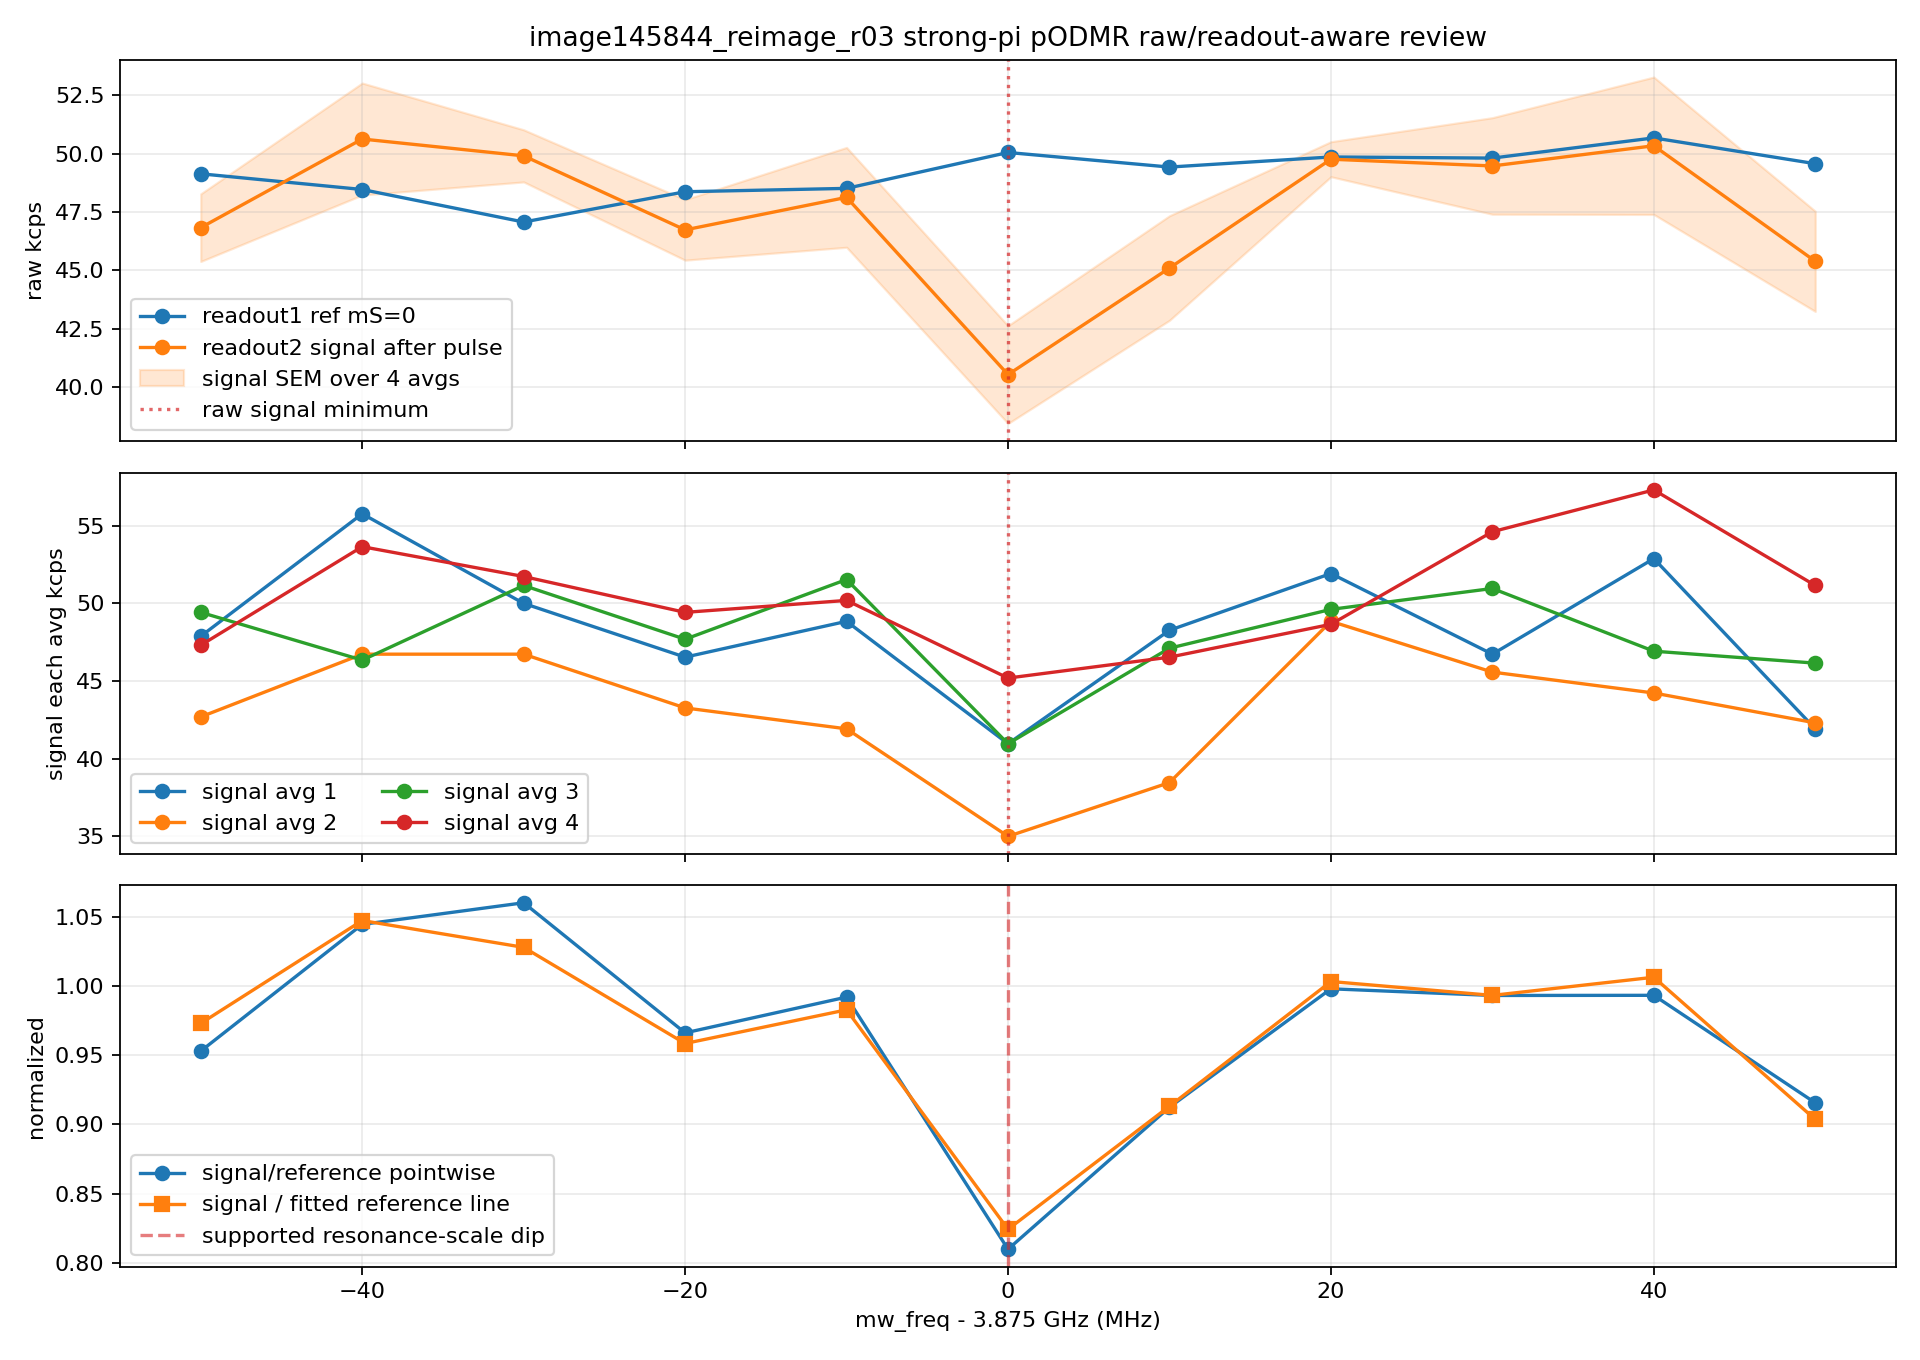
\includegraphics[width=0.88\linewidth,height=0.45\textheight,keepaspectratio]{figures/r03_strong_podmr.png}\\
{\small r03 strong-pi pODMR: alignment acceptance evidence.}
\end{center}

\begin{center}
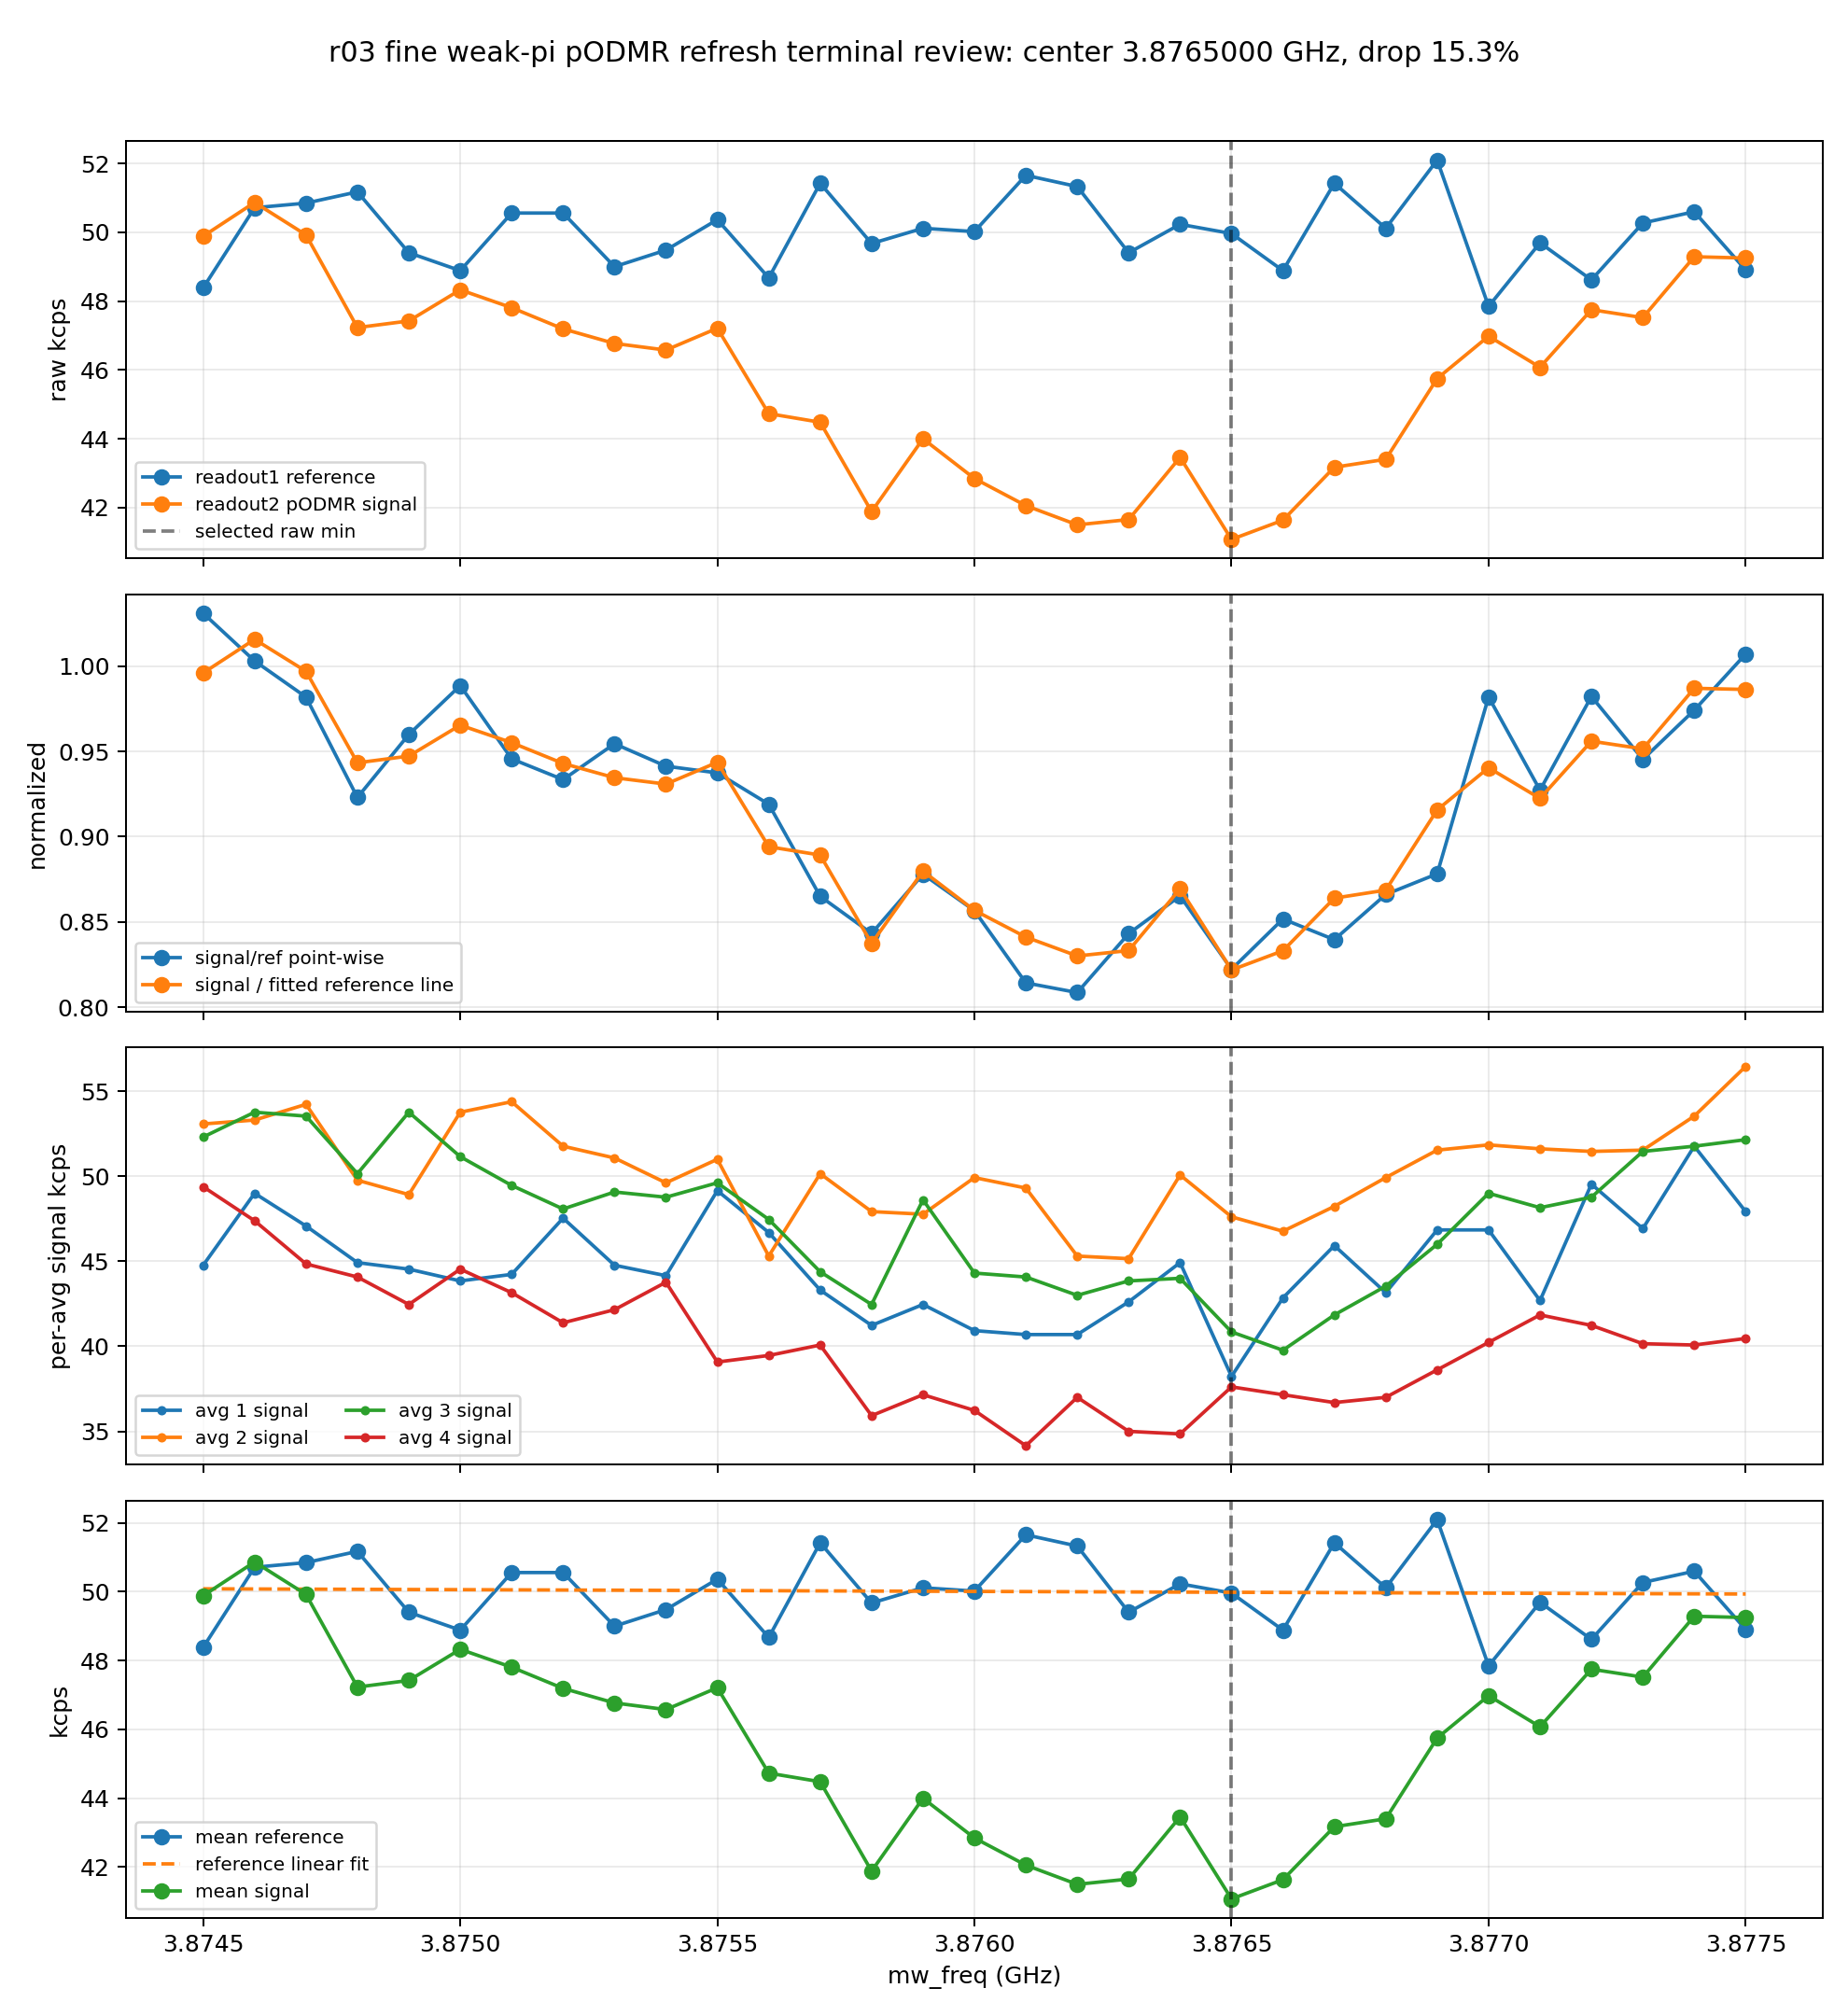
\includegraphics[width=0.88\linewidth,height=0.45\textheight,keepaspectratio]{figures/r03_podmr_refresh.png}\\
{\small Weak-pi pODMR refresh: grid-supported 3.8765 GHz resonance, with several-100-kHz calibration uncertainty.}
\end{center}

\begin{center}
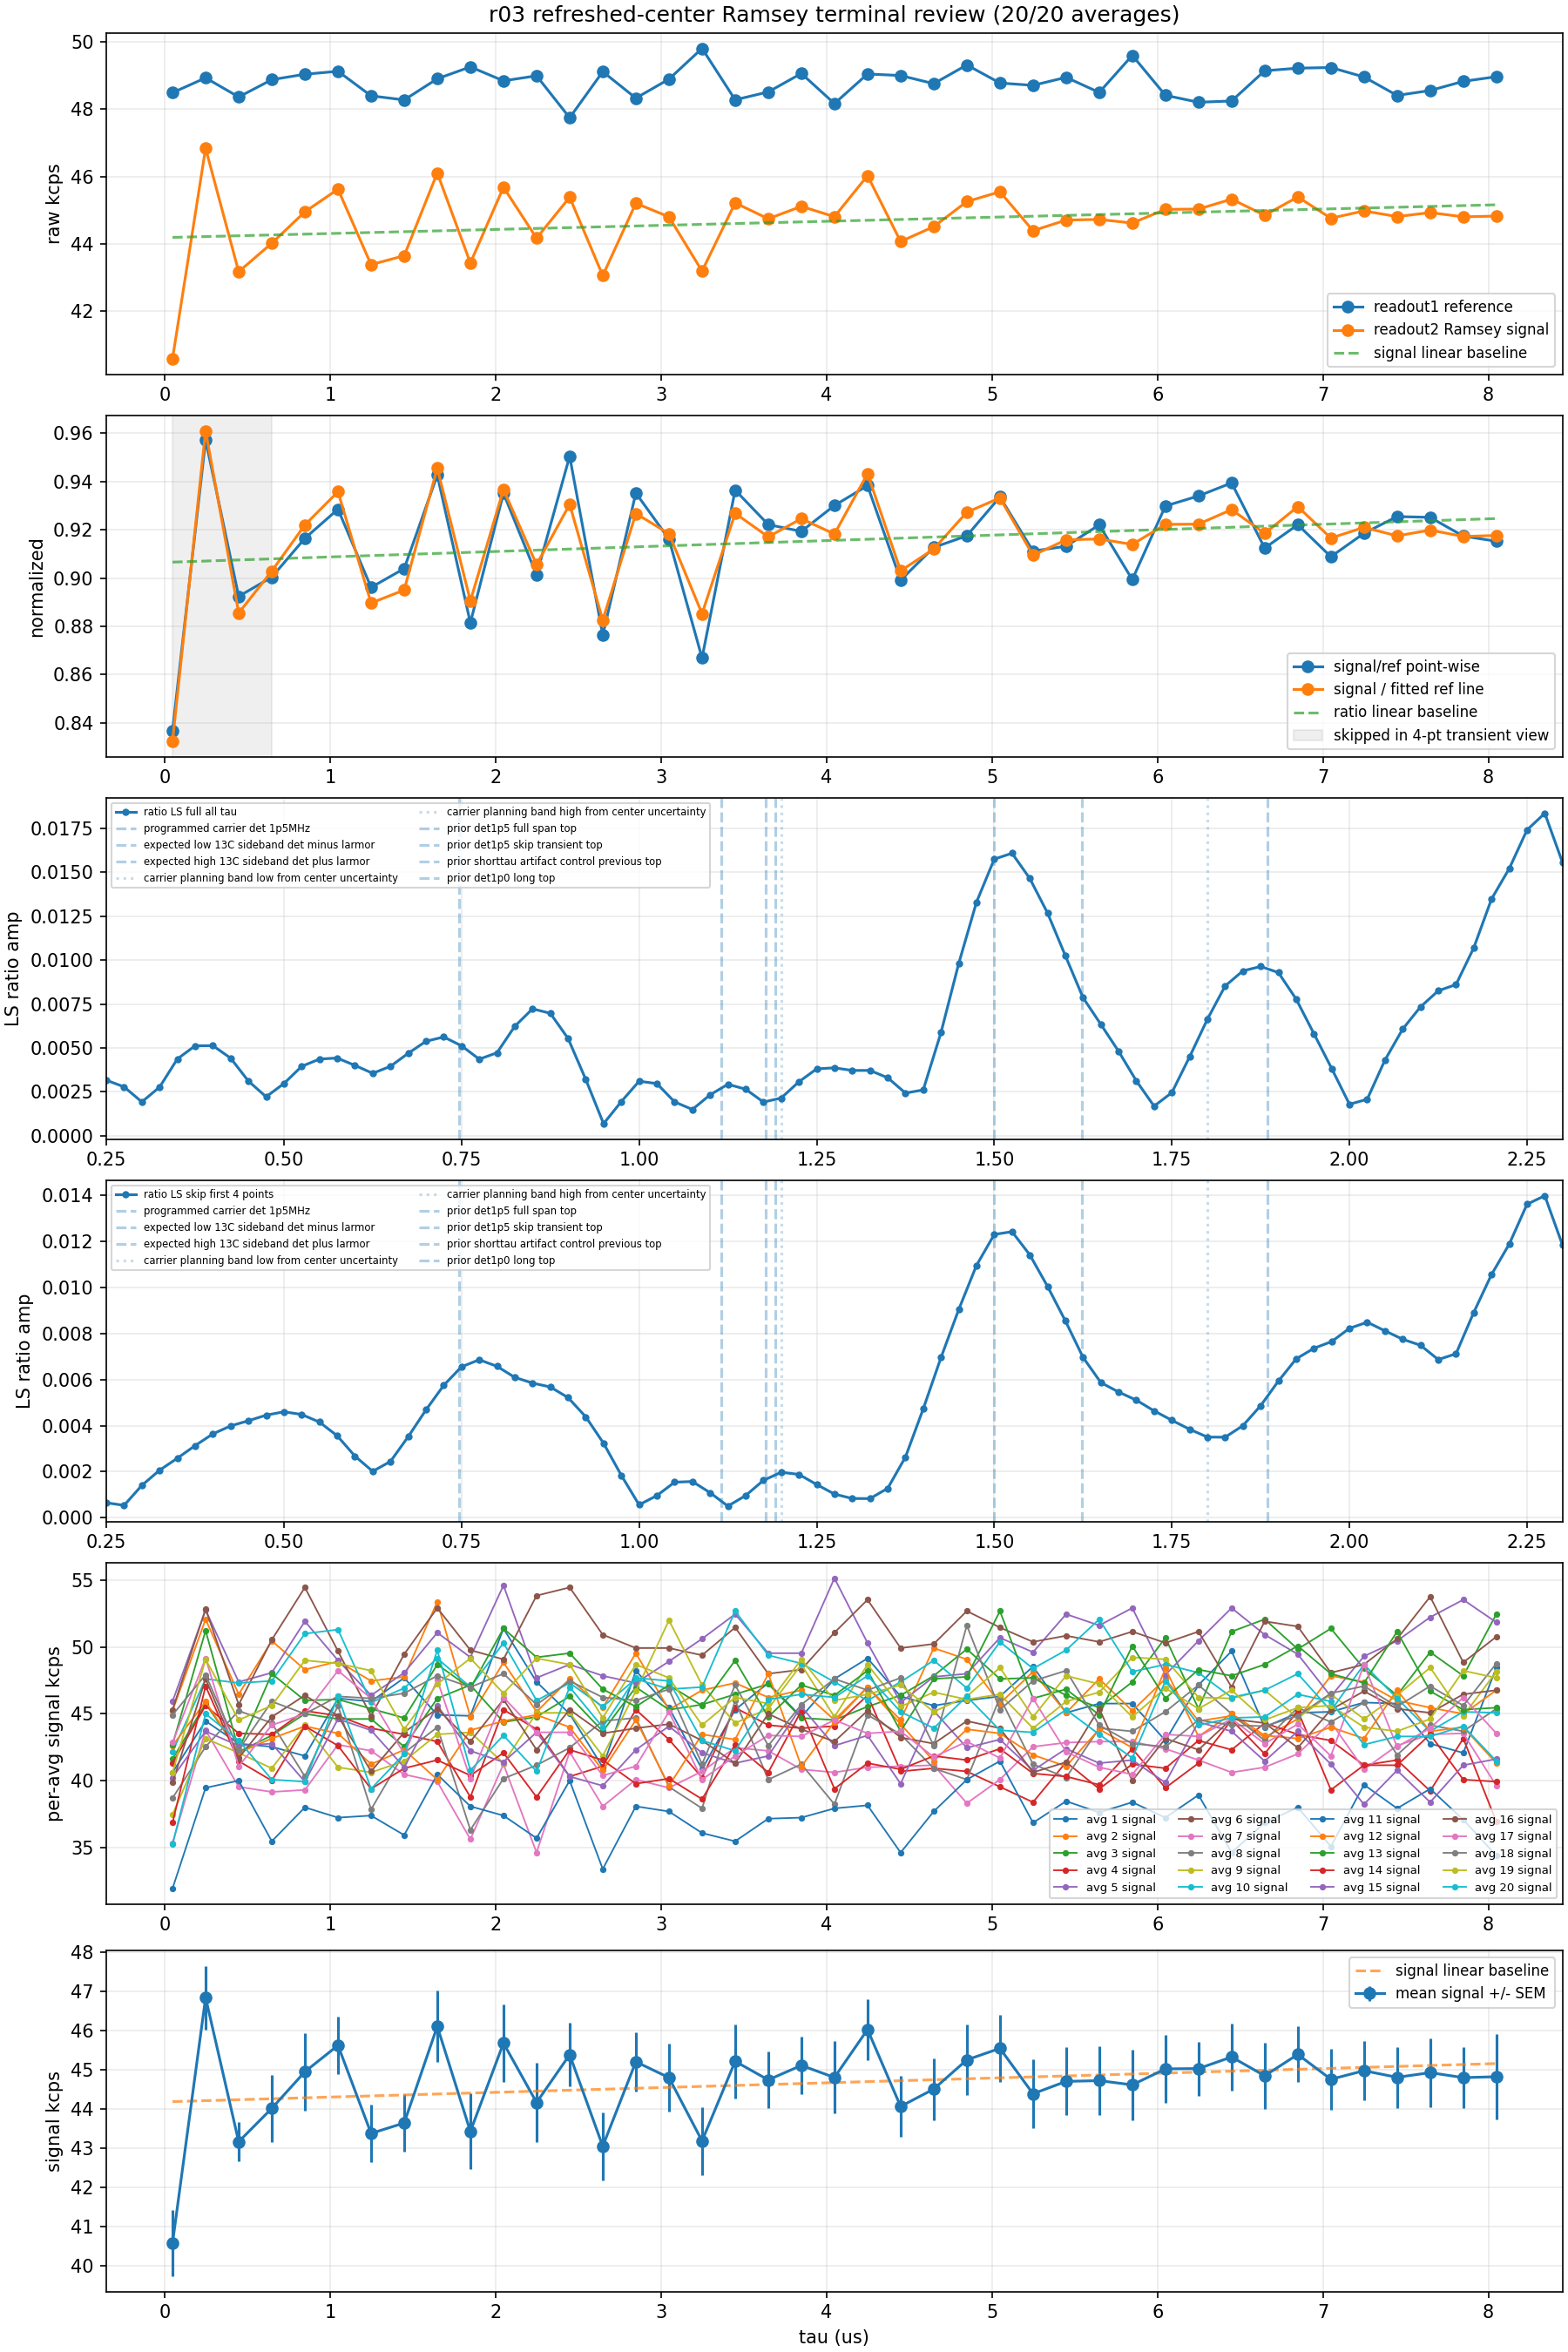
\includegraphics[width=0.88\linewidth,height=0.52\textheight,keepaspectratio]{figures/r03_final_ramsey.png}\\
{\small Terminal refreshed-center Ramsey data used for both the original and shifted-sideband analyses.}
\end{center}

\begin{center}
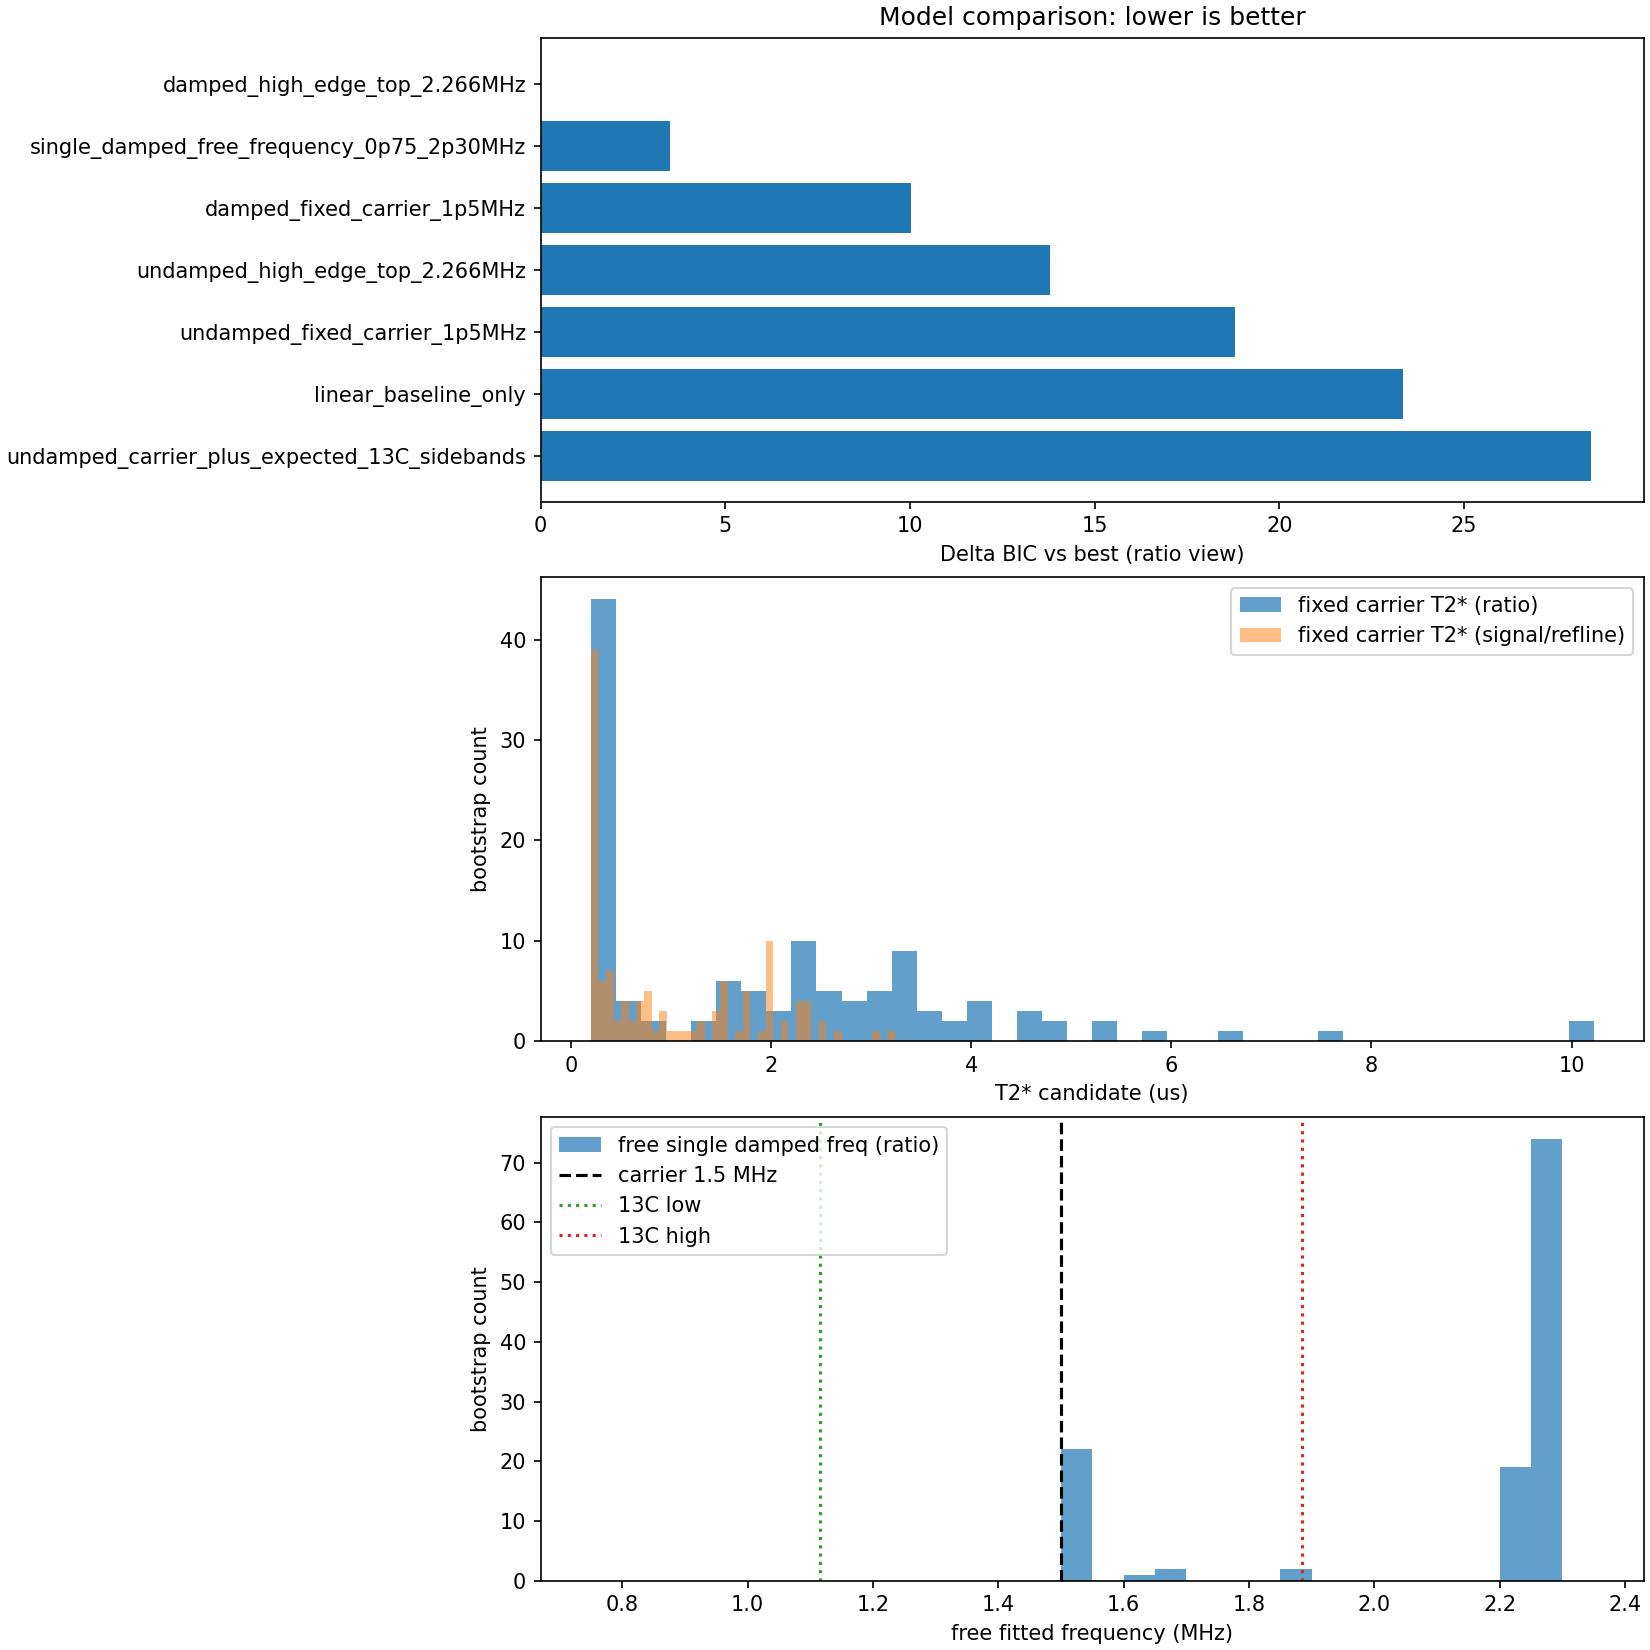
\includegraphics[width=0.88\linewidth,height=0.52\textheight,keepaspectratio]{figures/r03_original_model_comparison.png}\\
{\small Original fixed-carrier model comparison, before allowing a shifted carrier.}
\end{center}

\begin{center}
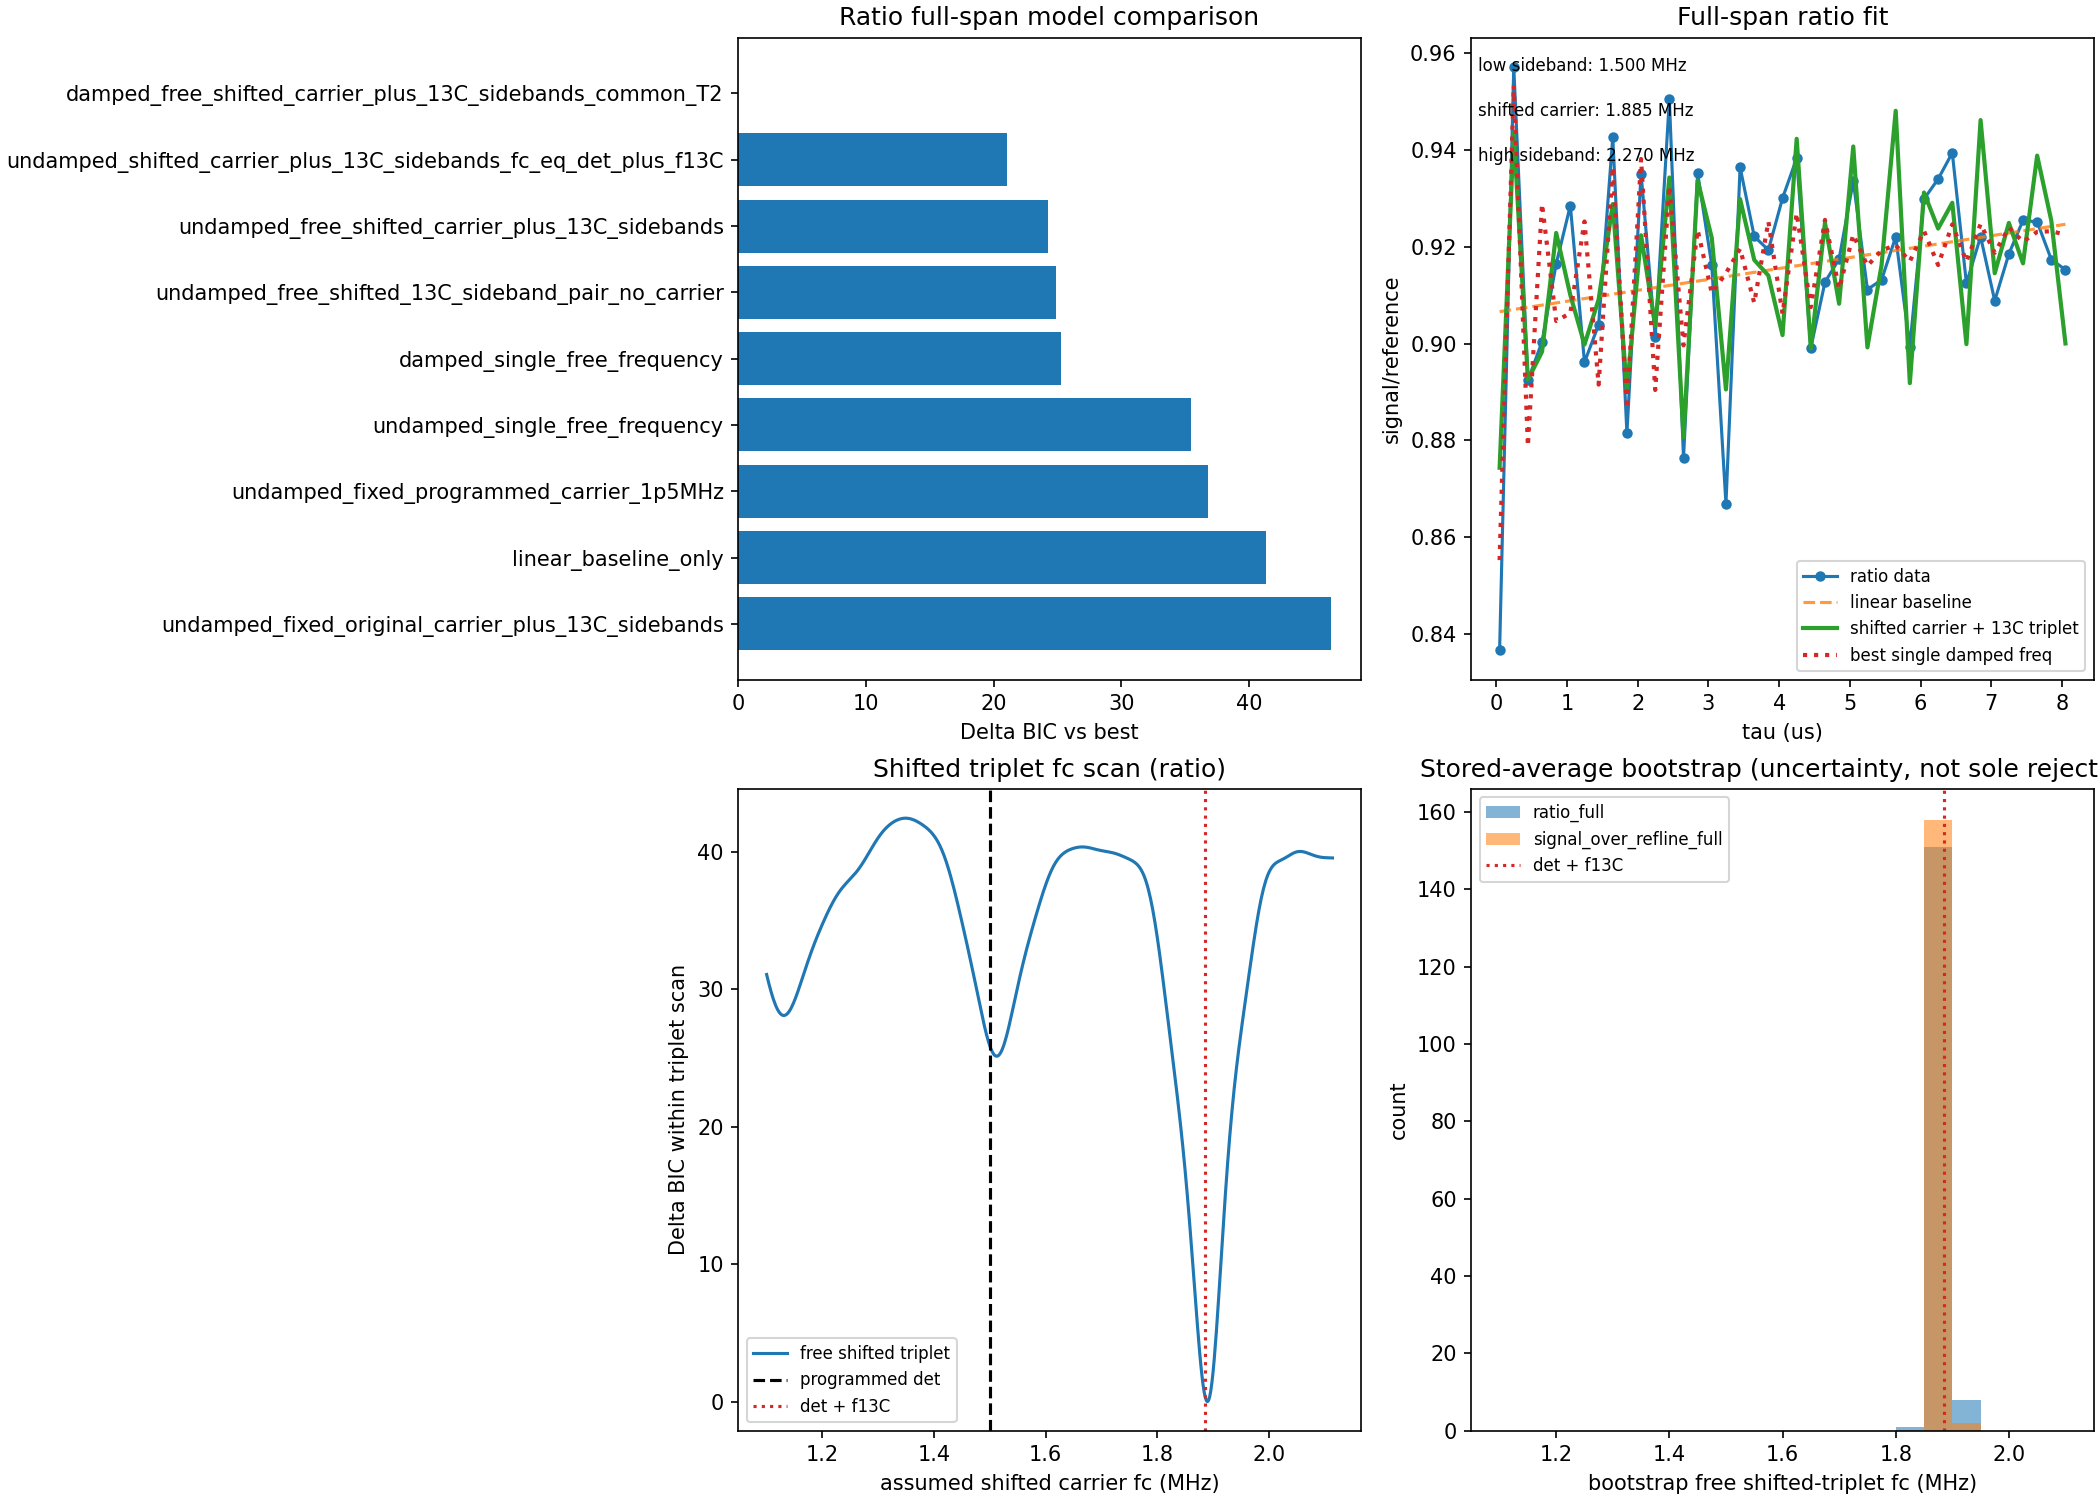
\includegraphics[width=0.88\linewidth,height=0.52\textheight,keepaspectratio]{figures/r03_shifted_sideband_reanalysis.png}\\
{\small Shifted-sideband reanalysis: the carrier-shifted triplet explains the 1.5/1.885/2.27 MHz pattern.}
\end{center}

\begin{center}
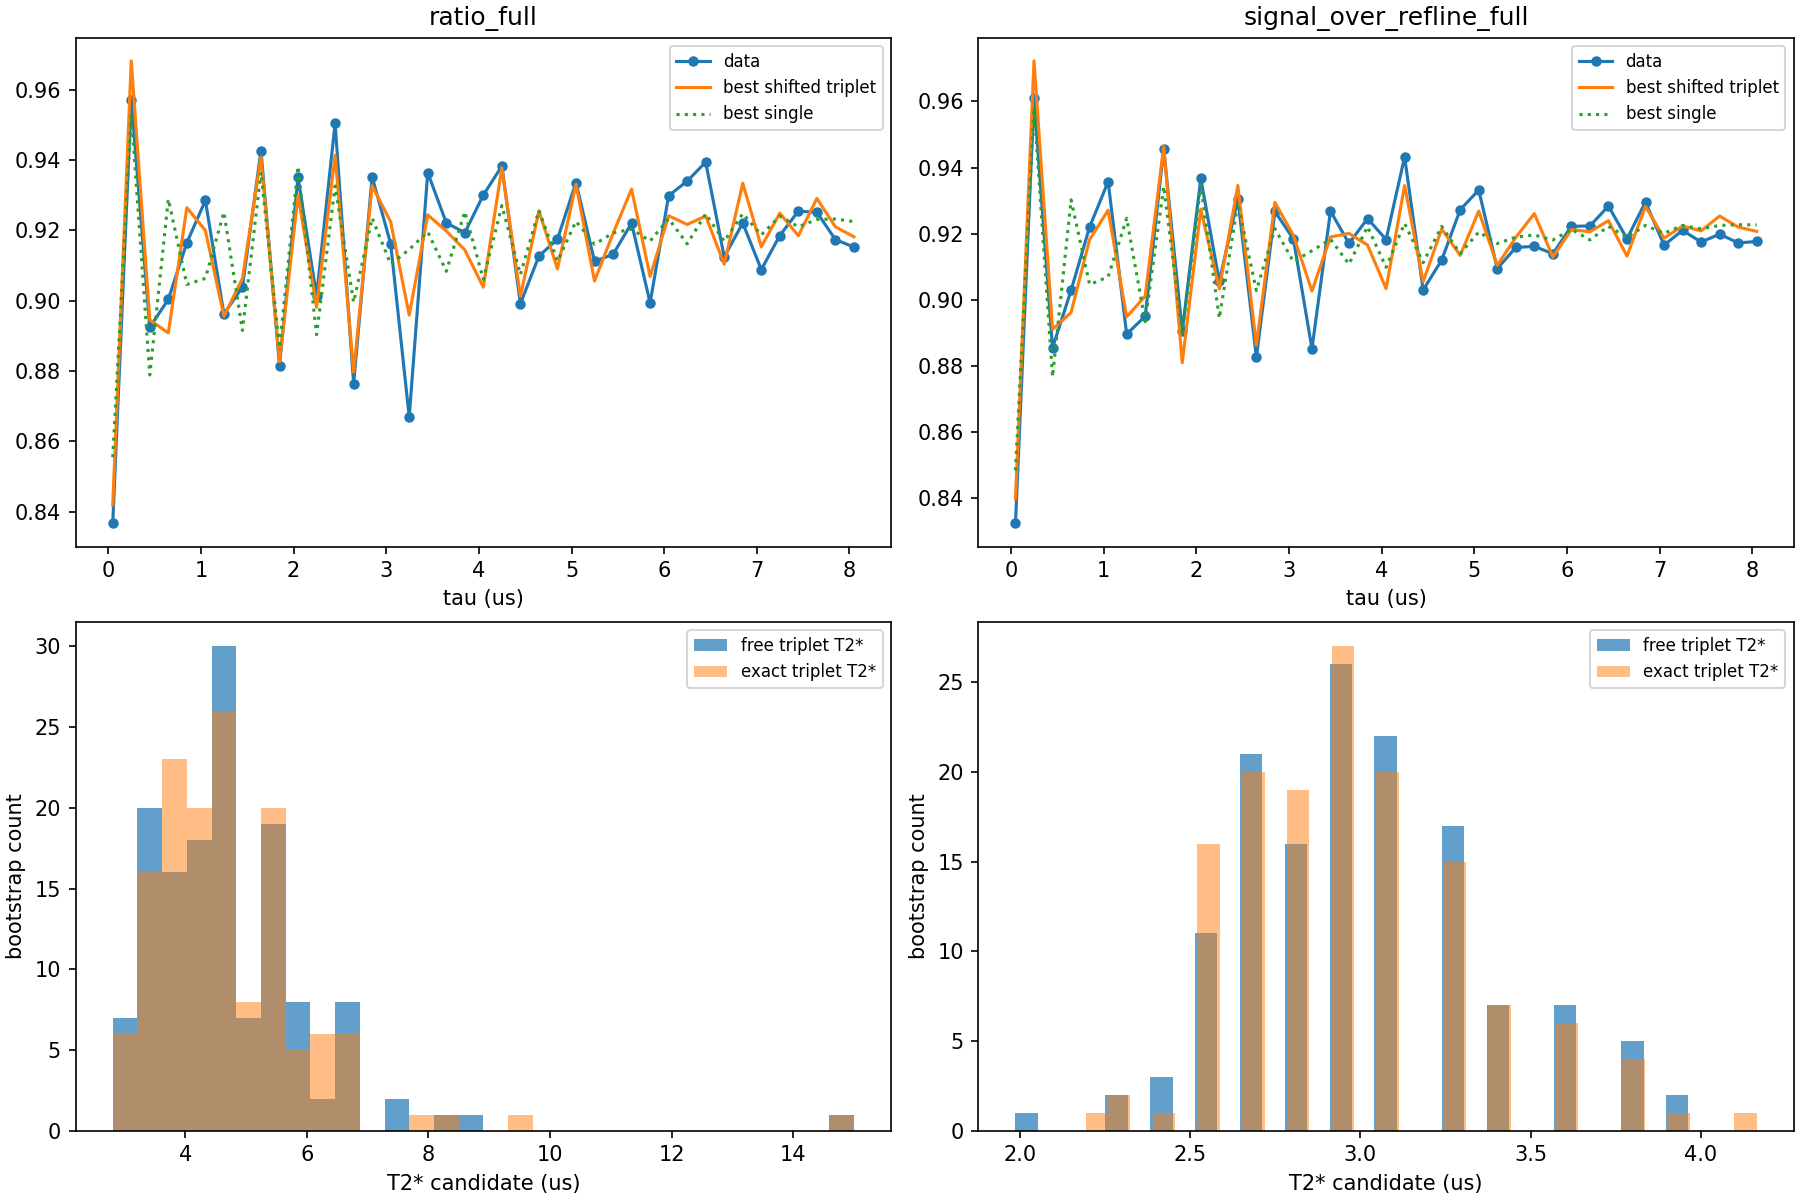
\includegraphics[width=0.88\linewidth,height=0.52\textheight,keepaspectratio]{figures/r03_shifted_triplet_bootstrap.png}\\
{\small Targeted bootstrap for the shifted triplet. Stored-average disagreement is treated as uncertainty, not as the sole rejection criterion.}
\end{center}

\section*{Revised project-scoped claims}
\begin{enumerate}
\item image145844\_reimage\_r03 is a magnetic-field-aligned NV candidate suitable for targeted follow-up.
\item The project does not establish an unconditional claim-grade numeric T2*. The best current shifted-triplet interpretation implies an order-3-us Ramsey decay scale, with targeted fits spanning about 2.7--4.6 us across robust views and bootstrap medians about 3--4.6 us.
\item The project does establish plausible candidate evidence for a nearby $^{13}$C-like shifted-sideband pattern in the final Ramsey, conditional on a residual carrier shift of about +0.39 MHz. This supersedes the earlier negative $^{13}$C wording but remains short of an independently confirmed coupling claim.
\end{enumerate}

\end{document}
